% Diagrama de Venn com dois conjuntos
% Feito para o ÉguaTeX (eguatex.com.br). Uso livre (CC0 1.0).
%
% Compile e pronto: sai só a figura, em PDF.
% Para pôr no seu trabalho, use o PDF com \includegraphics ou copie
% o bloco tikzpicture para dentro de uma figure.
\documentclass[tikz,border=4pt]{standalone}
\usepackage[T1]{fontenc}
\usepackage{lmodern}
\usepackage{amsmath}

\colorlet{corRegiao}{blue!35}

\begin{document}
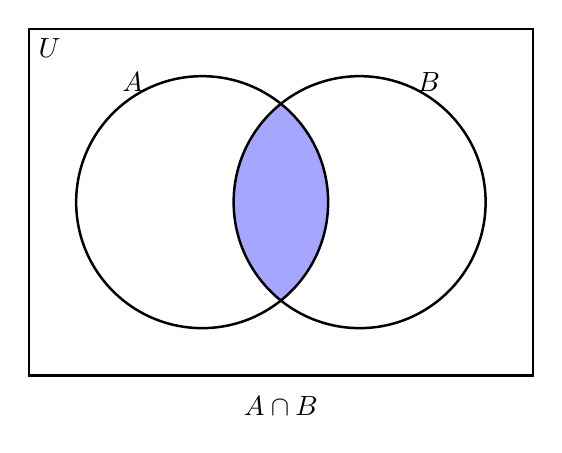
\begin{tikzpicture}[line cap=round]

% Mude estes números e textos.
\def\raio{1.6}         % raio de cada conjunto, em cm
\def\dist{2.0}         % distância entre os centros, em cm
\def\nomeA{$A$} \def\nomeB{$B$} \def\nomeU{$U$}
\def\legenda{$A\cap B$}

\def\conjA{(0,0) circle[radius=\raio]}
\def\conjB{(\dist,0) circle[radius=\raio]}
\def\universo{({-\raio-0.6},{-\raio-0.6}) rectangle ({\dist+\raio+0.6},{\raio+0.6})}

% Região pintada: deixe só uma das opções abaixo sem o % na frente
% e troque a legenda lá em cima pela da opção escolhida.
% Interseção, legenda $A\cap B$:
\begin{scope}\clip \conjA; \fill[corRegiao] \conjB; \end{scope}
% União, legenda $A\cup B$:
% \fill[corRegiao] \conjA; \fill[corRegiao] \conjB;
% Diferença, legenda $A\setminus B$:
% \begin{scope}[even odd rule]\clip \conjB \universo; \fill[corRegiao] \conjA; \end{scope}
% Complementar de A, legenda $A^{c}$:
% \fill[corRegiao, even odd rule] \universo \conjA;

% contornos e nomes
\draw[line width=0.9pt] \universo;
\draw[line width=0.9pt] \conjA;
\draw[line width=0.9pt] \conjB;
\node[anchor=north west] at ({-\raio-0.6},{\raio+0.6}) {\nomeU};
\node at ({-0.55*\raio},{0.95*\raio}) {\nomeA};
\node at ({\dist+0.55*\raio},{0.95*\raio}) {\nomeB};
\node[below=4pt] at ({\dist/2},{-\raio-0.6}) {\legenda};
\end{tikzpicture}
\end{document}
